\begingroup % keep various changes local

\def\;{\protect\it}
% It seems \chapter* doesn't support specifying a running head/toc
% entry via oparg. So we use a trick to style the appendix author
% properly. This defines the styling on the opening page:

\def\appendixauthor{\break\vbox to 30pt{}{\Large \mdseries by {\bf Jeremy Gray}}}

% and this changes it in the table of contents:

\addtocontents{toc}{\protect\def\protect\appendixauthor{\\by Jeremy Gray}}

% Finally, the left running head is set via \markboth (as usual, the right
% running head is reset by \section)

\chapter*{Appendix: A historical essay on some topics in algebraic
geometry \protect\appendixauthor}

\markboth{Appendix: A historical essay, by Jeremy Gray}{}

% \addAtotocsection is defined elsewhere; it formats the section
% number as A.number
\addtocontents{toc}{\begingroup \protect\addAtotocsection}

\setcounter{section}{0}
\setcounter{footnote}{0}
\setcounter{figure}{0}
\def\thechapter{A}
\def\thesection{\arabic{section}}

\quad\vskip-80pt%
\noindent(Open University, Milton Keynes, United Kingdom)
\vskip30pt

\label{Appendix-History}
This essay offers a brief overview of aspects of the long history of
plane curves and algebraic geometry.%
\index{historical context|(}%
%
\footnote{I am grateful to Andrea
del
\index{Centina@del Centina, Andrea}%
Centina for letting me read the manuscript of his forthcoming book
\emph{The History of Projective Geometry}, which has been very helpful
and will surely become the definitive work on the subject.}
%
It starts
with some historical remarks about conic sections, moves on to look
at some aspects of the early study of cubic and quartic curves and
the emergence of real and complex projective space, then nods briefly
at Bernhard Riemann's ideas about algebraic curves and Luigi Cremona's
ideas about plane transformations before concluding with an introduction
to the work of Alexander Brill and Max Noether in the late 19th century.

\section{Greek mathematicians and conic sections}

Quadratic problems were part of high-level teaching in ancient
Mesopotamia
\index{Mesopotamia}%
around 1800 BCE. One such tablet (BM 13901) begins%
%
\footnote{This is
tablet number 13901 in the British Museum collection.}
\begin{quote}
I have added up the area and the side of my square: 0;45.
\end{quote}
The unstated task is to find the side of the square.
The number 0;45 is $\ssty\frac{\ssty3}{\ssty4}$ in sexagesimal notation,
so if we rewrite this as an equation for $s$, the unknown side, we have
$$s^2 + s = \tsty\frac{3}{4}.$$
The tablet then goes through the steps of an algorithm much as we would
for finding the positive root: $s = \haa$.

Other problems involve knowledge of the Pythagorean
\index{Pythagorean theorem}%
theorem, known also
to Chinese and Indian mathematicians. But the first mathematicians to
have studied curves more complicated than the straight line and the
circle seem to have been those of ancient Greece.  Surviving sources
suggest that the study of conic sections,
\index{conic section}%
\index{Greek mathematics}%
literally sections of a cone,
may well have arisen with Menaechmus's
\index{Menaechmus}%
work on doubling the
\index{doubling the cube}%
cube around
350 BCE. This was a long-standing problem that was given a theological
spin in the form of the Delian problem, which, according to one story,
asked for an altar double the size of a given one, apparently to get
rid of a plague. Finding this difficult, workers consulted Plato, who
said that the real reason for the task was to reproach the Greeks for
their neglect of geometry.%
%
\footnote{Theon of Smyrna, 
\index{Theon of Smyrna}%
2nd century CE, in (Thomas 1939, Vol.\ 1, 257).}
%
It may well also have stood out because Plato
\index{Plato}%
in the \emph{Meno}
dialogue made such a fuss of doubling the square. Hippocrates of
Chios,
\index{Hippocrates of Chios}%
who flourished around 470 BCE,  had already reduced the
cube doubling
problem to that of finding two mean proportionals between 1 and 2;
i.e., quantities $x$ and $y$ such that
\begin{equation}\label{Menmus}
1:x= x:y = y: 2.
\tag{$*$}
\end{equation}
For Greek mathematicians, these quantities would have been line segments
of those lengths.

Many solutions to the problem of finding two mean proportionals were
proposed.
Menaechmus, a younger associate of Plato and a pupil of Eudoxus,
\index{Eudoxus}%
may
have been the first to connect the problem of doubling the cube to the
idea of conic sections, or perhaps we should say quadratic curves,
\index{quadratic curve}%
because it has been argued that he considered equation \eqref{Menmus}
as defining or generating curves that would have been drawn and
understood pointwise. At all events, he expressed the solution to the
Delian problem in terms of the intersection of a hyperbola
\index{hyperbola}%
and a
parabola.
\index{parabola}%
%
\footnote{See Eutocius 
\index{Eutocius}%
\emph{Commentary on Archimedes' Sphere
  and Cylinder}, in (Cohen and Drabkin 1948, 62--66).
  Among Eudoxus's many achievements is to have provided the first
  theory of
  magnitudes that went beyond the rational numbers; it is now found in
  Book V of Euclid's
\index{Euclid}%
\emph{Elements}.}

About a century after Menaechmus' time, Diocles,
\index{Diocles}%
 and soon
after him Apollonius
\index{Apollonius}%
 made significant progress with the conic
sections.%
%
\footnote{The first places to go for an account of Greek
mathematics are the analytical account in (Netz 2022) and the detailed
if sometimes dated century-old account (Heath 1921).}
%
Diocles identified the curve that would focus the sun's rays to a point
as the parabola, and knew precisely how to cut a cone so as to obtain it.%
%
\footnote{Apollonius's four books of his conics survive in Greek and
three more in Arabic; the eighth and final volume is lost.}


Apollonius produced the first \emph{theory} of conic sections
\index{conic section!theory of --s}%
as sections
of a cone.
The books are very dry. Van der Waerden
\index{Van der Waerden, Bartel Leendert}%
called him a virtuoso ``in dealing
with geometric algebra, and also a virtuoso in hiding his original line
of thought'', while going on to say that ``his reasoning was crystal
clear and elegant.''%
%
\footnote{See (Van der Waerden 1961, 248).}
%
Apollonius began with the basic definitions of a cone (on a circle)
and its three types of section: the hyperbola, parabola, and ellipse;
\index{ellipse}%
the names are due to him. He showed that all the known sections that
had been studied as sections of a cone with vertical angle a right angle
could be obtained as sections of a suitable but otherwise arbitrary cone.

It's  arguable that a system of
\index{coordinate system}%
coordinates was present in his work,
inasmuch as he generally referred everything to a pair of distinguished
lines in the plane of section of the cone, but it is buried in the heavy
use of proportion theory between different line segments.
Apollonius produced a theory of the principal diameters
\index{principal diameter}%
of conics, studied
such problems as finding the tangents to a
\index{tangent}%
\index{conic!tangent to}%
conic from an exterior point,
and came close to observing the properties of cross-ratio that modern
writers were to detect. He also had a theory about normals to conics
\index{normal!to a conic}%
from which  it's a short step to obtaining their evolutes.
The biggest weakness in his theory was that very often he had to treat
the three kinds of conic section separately, although you can see him
trying for greater generality, as, for example, when he introduced the
concept of conjugate hyperbolas in Book I to make the proofs of theorems
about conjugate diameters run equally elegantly and simply for hyperbolas
as ellipses.




Mathematicians of the Islamic
\index{Islamic mathematics}%
era  (active from the 9th to the 15th
century CE)
also studied conic sections and the various problems they inherited from
the Greeks. One of the most outstanding is `Umar ibn Ibr\={a}h\={i}m
al-Kh\={a}yyam\={i} (usually known in the West as Omar Khayy\={a}m),
\index{Khayy\={a}m, Omar}%
\index{al-Kh\={a}yyam\={i}, Umar ibn Ibr\={a}h\={i}m}%
who was born in Nishapur in northern Iran  in the 11th century CE and
spent much of his life in Isfahan, where he led a group of Islamic
astronomers at the observatory there. In his book the \emph{Ris\={a}la} he
 gave a complete account of how to solve cubic equations
\index{cubic equation, geometric solution}%
using pairs
 of conic sections where necessary.%
\footnote{See (al-Kh\={a}yyam\={i} 1950).} 
%
Other Islamic mathematicians advanced the study of trigonometry,
\index{trigonometry}%
investigated the foundations of geometry (Euclid's parallel postulate
\index{parallel postulate}%
\index{Euclid}%
(which al-Kh\={a}yyam\={i} also investigated), invented methods for
the numerical solution of polynomial equations,
\index{polynomial equation, numerical solution}%
and studied various
properties of conic sections, but there was little study of other kinds
of curves.

\section{The first appearance of complex numbers}
In the 16th century, various Italian mathematicians, notably Gerolamo
Cardano,
\index{Cardano, Gerolamo}%
Ludovico Ferrari,
\index{Ferrari, Ludovico}%
and Rafael Bombelli,
\index{Bombelli, Rafael}%
succeeded in finding
algebraic methods for solving cubic and quartic equations. This inevitably
led them to have views about complex numbers.
\index{complex numbers}%
 Cardano recognised in
his  (1545, Chapter\,37) that they will appear in the formulae for
the solution of these equations, even though he said ``So progresses
arithmetic subtlety, the end of which, as is said, is as refined as it is
useless.'' Bombelli was more hospitable to the new numbers in his  (1572),
and gave rules for manipulating them, but they remained mysterious and
suspect for many years.



At this point, the history of algebraic geometry broadly divides into
two. One part concerns the theory of conic sections\emdash algebraically,
curves of degree two\emdash and the other the theory of curves of higher
degree. The first can regard Girard Desargues
\index{Desargues @Desargues, Girard}%
as a major innovator,
the second his contemporary,  Ren\'e Descartes.
\index{Descartes, Ren\'e}%
Together, they lead
to the concept of a projective space. Let us take the study of conic
sections first.


\section{Conic sections from the 17th to the 19th centuries}
In 1639 Desargues published fifty copies of a short pamphlet known as
the \emph{Brouillon Project}
\index{Brouillon Project}%
 (1639), on what we could call the
projective theory of conics. He was perhaps hoping for useful critical
feedback, but he never returned to rewrite his account.  In the essay,
all non-degenerate conics are treated on a par, and treated as
\index{projective geometry}%
perspective images of the circle. The idea that all (non-degenerate)
conics are the projective image of a circle is not original with
Desargues. It was stated by Francesco Maurolico,
\index{Maurolico @Maurolico, Francesco}%
 for example, in his
book  (1611), which it is likely Desargues knew, and in any case it is
visually apparent to anyone who thinks of the conics as sections of a
cone on a circular base. The trick is to make this insight work.

Desargues's key idea is that of properties of figures invariant under
projection, such as the cross-ratio
\index{cross-ratio}%
of four points on a line: if $A,
B, C, D$ are four points on a line, their cross-ratio can be defined to be
$\unfrac{(AC.DB)}{(AD.CB)}$. The special case,  when the cross-ratio
is $-1$ and $AC/CB=-AD/DB$ and people said $B$ and $D$ separate $A$
and $C$ in the same ratio, arises frequently in the theory of the
poles and polars of conic section.%
%
\footnote{Desargues did not use the
  concepts of pole and polar but of four or six points in involution.}
%
Desargues also had a more complicated property of six points, which,
like the four-point property, was invariant under a projection. He
connected all this to the study of the ``complete quadrilateral''
\index{complete quadrilateral}%
(see
Figure \ref{figCompleteQuad})\emdash take four points, no three
collinear, and join them in all possible ways\emdash  and thence to
the study of conics through those four points.

\begin{figure}
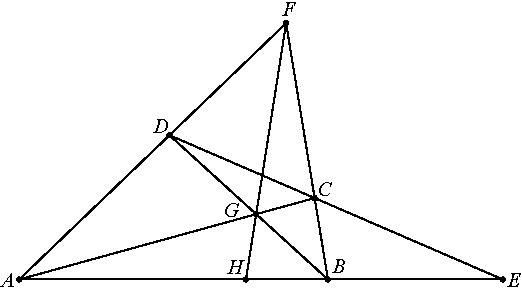
\includegraphics[width=200pt]{main/CompleteQuad3}
\caption{A complete quadrilateral, consisting of the four points $A, B,
C, D$ and the three lines joining them in pairs.}
\index{complete quadrilateral}%
\label{figCompleteQuad}
\end{figure}


The  \emph{Brouillon Project} is fiercely unreadable.%
%
\footnote{Happily,
it has been the subject of sequence of detailed analyses in recent papers
by Marie  Anglade
\index{Anglade @Anglade, Marie}%
and Jean-Yves Briend;
\index{Briend Jean-Yves}%
 see (Anglade and Briend 2022)
and the references to their earlier papers cited there.} 
%
It was also lost
for a long time and known only through commentaries by later authors
until in 1845 Michel Chasles
\index{Chasles @Chasles, Michel}%
found a handwritten copy made by Philippe
de la
\index{Hire @Hire, Philippe de la}%
Hire.%
\footnote{The only known copy of the original \emph{Brouillon
project} turned up in 1950.}
%
In particular, de la Hire, a generation after
Desargues, wrote some much more readable, and longer, works in Desargues's
spirit, illuminating the role of cross-ratio in the theory of tangents
that came close to a theory of duality. Desargues's famous theorem
\index{Desargues theorem}%
on two triangles in perspective was published separately in (Bosse 1648).

The best attention Desargues's little book got was from his younger
contemporary Blaise Pascal,
\index{Pascal @Pascal, Blaise}%
 who evidently produced a virtually
complete theory of conics
\index{conics, theory of}%
around what he called the ``mystical hexagram''.
\index{mystical hexagram}%
 Unhappily, much of it is lost, and known to us only from
some notes on it made by Leibniz,
\index{Leibniz @Leibniz, Gottfried Wilhelm}%
but the idea is that while there is
always a conic through five points something happens if you want a conic
through six points: we call it Pascal's theorem.
\index{Pascal's theorem}%
 Then, if you let the
sixth point collapse onto one of the other five you get a tangent to the
conic through those five points. One way or another all the key properties
of conics are wrapped up in this idea, or so Pascal seems to have shown,
and much of the early 19th century work in France can be seen as attempts
to recover such a theory, which would include such topics as duality,
\index{duality}%
in the form of the pole and polar
\index{pole and polar relative to a conic}%
\index{conic!pole and polar}%
relationship with respect to a conic
(see Figure \ref{figpolepolar}).%
%
\footnote{For a thorough analysis of
\index{Centina@del Centina, Andrea}%
Pascal's work and its context, see (Del Centina 2020).}

\begin{figure}
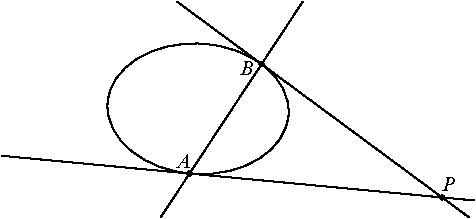
\includegraphics[width=180pt]{main/poleandpolar}
\caption{The tangents from a point $P$ outside the conic touch it at
  $A$ and $B$; the line $AB$ is the \emph{polar} of $P$ and $P$ is the
  \emph{pole} of the line $AB$. The construction can be extended to
  points inside the conic.}
\index{pole and polar relative to a conic}%
\index{conic!pole and polar}%
      \label{figpolepolar}
\end{figure}

Thereafter, truly projective geometry
\index{projective geometry}%
languished for much of the 18th
century, despite some insightful contributions by Isaac Newton that we
shall mention below (see p. ~\pageref{Newtonconics}) and a few others. Its
revival is conventionally dated from the early work of Gaspard Monge,
\index{Monge @Monge, Gaspard}%
who as a young man seeking a job in the French army was  interested in
how to depict three dimensions on two. He devised a method of plan and
elevation
\index{plan and elevation}%
(projections onto a horizontal and a vertical plane) that he
could couple to some simple algebra in a way that was easy to use; as a
result he was offered a job at the military Academy in M\'ezi\`eres
%\index{M\'ezi\`eres military Academy}%
and
his discovery made a military secret. During the French Revolution, Monge
was influential in setting up the \'Ecole Polytechnique,
\index{Ecole@\'Ecole Polytechnique}%
 where he was
an inspiring teacher of geometry, and this did much to revive the subject.

Among those so inspired there was Jean Victor Poncelet,
\index{Poncelet @Poncelet, Jean Victor}%
 who promoted
\index{porism, Poncelet}%
a much more general theory of transformations with a view to unifying
the theory of conics that he began to develop while a prisoner-of-war
in Saratov during Napoleon's disastrous invasion of Russia. His
\emph{Trait\'e des Propri\'et\'es Projectives des Figures} (1822) is a
visionary book that relies on some rather mysterious arguments about ideal
points of intersection (Augustin-Louis Cauchy,
\index{Cauchy @Cauchy, Augustin-Louis}%
 who reviewed the book,
urged that they be regarded as points with complex coordinates;
\index{complex numbers}%
 Poncelet
never agreed, and reproduced the review between the Preface and the
Introduction to his \emph{Trait\'e}  presumably to show his disdain). As
a result, some of the transformations it invokes necessarily require
complex coordinates. The most famous result in the book is Poncelet's
closure theorem,
\index{closure theorem (Poncelet)}%
 which has continued to attract attention to this day,
but it is also notable for many other theorems involving pairs of conics.


In the 1820s, Poncelet had a dispute with Joseph Diaz Gergonne,
\index{Gergonne @Gergonne, Joseph Diaz}%
 the editor
of the only journal at the time entirely devoted to mathematics, about
what duality in the plane actually is.%
%
\footnote{Gergonne's journal was
called the \emph{Annales de Math\'ematiques Pures et Appliqu\'ees}. It ran
\index{Annales@\emph{Annales de Math\'ematiques Pures et Appliqu\'ees}}%
from 1810 to 1832, and  it was succeeded in by Liouville's
\index{Liouville @Liouville, Joseph}%
\emph{Journal
\index{Journal@\emph{Journal de Math\'ematiques Pures at Appliqu\'ees}}%
de Math\'ematiques Pures at Appliqu\'ees} in 1836. Crelle's
\index{Crelle @Crelle, August Leopold}%
\emph{Journal
\index{Journal@{\;Journal f\"ur die reine und angewandte Mathematik}}%
f\"ur die reine und angewandte Mathematik} was founded in 1826.}
%
Poncelet always saw it as pole and polar with respect to a conic,
Gergonne saw it as a new and fundamental feature of projective
\index{projective geometry}%
geometry.%
%
\footnote{See (Gergonne 1826).} 
%
Gergonne's view led to confusion
when it was applied to curves of degree three or more, a matter that began
to be sorted out only with Julius Pl\"ucker's work, as we shall see below.


Another mathematician who was inspired by Monge was Michel Chasles,
\index{Chasles @Chasles, Michel}%
who used the projective invariance of the cross-ratio of four points
to eliminate much of the weirdness of Poncelet's ideas. Independently,
Jakob Steiner
\index{Steiner @Steiner, Jakob}%
did very similar work in Germany. He can be credited
with the first truly projective definition of a conic section.
\index{conic!projective definition}%
 Even so,
there remained an irritating feature of cross-ratio:
\index{cross-ratio}%
 it was given as a
function of four lengths, but length is a property of Euclidean geometry,
not projective geometry.  If projective geometry is to be regarded as
more fundamental than Euclidean geometry, because it rests on fewer
assumptions or axioms, then the intrusion of Euclidean length in the
definition of cross-ratio is at the very least unfortunate. Nor can one
easily speak of there being a concept of projective space in the 1820s;
rather, much of geometry at this time was about figures in the plane
subject to a variety of projective transformations. The first truly
foundational work on real and complex projective geometry that avoided
deriving it from Euclidean geometry
\index{projective geometry!versus Euclidean}%
was the achievement of Karl von Staudt
\index{Staudt, Karl von}%
in his \emph{Geometrie der Lage} (1847), a long and difficult work that
influenced Felix Klein
\index{Klein @Klein, Felix}%
when he succeeded von Staudt as a Professor at
\index{Erlangen University}%
Erlangen twenty-five years later.%
%
\footnote{See, for example, (Gray 2015).}

All in all, a surprising amount of work was done on the theory of conic
sections  at the start of the 19th century, and before it is dismissed
as arcane it should be stressed that the subject was a proving ground
for the development of projective geometry.
\index{projective geometry}%
 Two approaches stand out: the
search for entirely  general methods that would treat all non-degenerate
conics on a par; and the emergence of the property of duality. Matters
\index{duality}%
are complicated by the existence of two separate traditions, usually
called the synthetic
\index{synthetic geometry}%
\index{analytic geometry}%
and the analytic, supposedly divided into classical
geometric methods and more algebraic ones that introduce coordinates.
Recent historical work suggests that it was all a bit murky, and algebraic
methods were also often used in synthetic geometry.%
%
\footnote{See (Lorenat 2016).} 
%
Several things promoted the use of synthetic methods. They can
be elegant when algebraic methods are blunt; they correspond to the
visual form of the conics; they provide a language for describing what
is apparent or to be found in a problem. Against them is the obstinate
fact that algebra is more general: it does not care if some quantities
become negative, but what is a negative length? Once ways round this
obstacle were found (by Poncelet and then Chasles) the way was open to
a truly systematic synthetic theory of conics.

How then did this change, and purely synthetic projective geometry
\index{projective geometry!synthetic versus analytic}%
begin to wane? Very few of the original protagonists disdained algebra
outright, and as the (projective) theory of conics reached completion in
the 1820s and established its fundamental character, being more general
than metrical Euclidean geometry, it also had its baroque aspects. But
worse, it did not generalise at all readily  to the study of curves of
higher degree. For that, as even Newton had recognised, a hefty dose of
algebra was required.


\section{Curves of higher degree from the 17th to the early 19th century}
A common way to think of curves in antiquity was pointwise: some length
depends in a given way on some other length. Accordingly, at least in
principle, if you know the independent length
(the ordinate, or $x$ coordinate)
\index{coordinate system}%
 you know the dependent length (the
abscissa, or $y$ coordinate).

By Descartes' time there was already some sophisticated algebra expressed
in a formalism that hadn't quite shaken off   the Greek insistence on
seeing everything as geometrical magnitudes: lengths, areas, volumes, and,
well, what exactly? The French mathematician Fran\c{c}ois Vi\`ete
\index{Vi\`ete, Fran\c{c}ois}%
in his
\emph{Isagoge} boldly spoke of magnitudes having the dimensions of side,
square, cube, square-square,
\index{square-square, square-cube}%
 square-cube and so on.%
%
\footnote{See his collected works, (Vi\`ete 1646).} 
%
It was possible to write polynomial
equations in this language, as Vi\`ete did in the early 1600s. First
Fermat
\index{Fermat @Fermat, Pierre de}%
in 1636, and then much more boldly Descartes
\index{Descartes, Ren\'e}%
in 1637, realised
that you could extend the language to two variables and so describe
curves in the plane.


\begin{figure}
  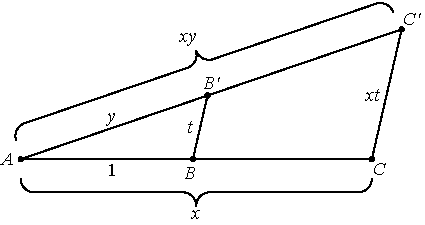
\includegraphics[width=180pt]{main/Multiplication}
\caption{If $AB$ is of length 1, $AC$ of length $x$, $AB'$ of
length $y$, and $BB'$ and $CC'$ are parallel then $AC'$ is of length $xy$.
}
      \label{figmultiplication}
\end{figure}

Descartes's first achievement in his \emph{La G\'eom\'etrie} (1637)
was to eliminate the dimensional
\index{dimensionality}%
aspect. A simple use of similar
triangles allowed him to show that the product of two lengths could
be seen as another length (not an area) so all geometrical quantities
could be regarded as one-dimensional and the idea of dimension quietly
dropped (see Figure \ref{figmultiplication}). He also replaced Vi\`ete's
cumbersome algebra, which was written in capital letters with verbal
abbreviations for the algebraic operations, with something much more like
what we use today.  He wrote $x$ and $y$ for the key variables (not $A$
and $E$ in the manner of Vi\`ete). Descartes was clear that he was using
\index{coordinates system}%
coordinates, although his $x$ and $y$ coordinates could have oblique axes.


Then came the real work. Almost all mathematical problems in his day
were expressed in the language of geometry, except for some that
we would call diophantine
\index{diophantine problems}%
and were implicitly about integers and
rational numbers. Accordingly, the answer had to be expressed
geometrically. Descartes's idea was to give letters to all the lengths
involved in a problem, use the statement of the problem to express
relationships between the letters, and reduce the equations to a
single equation. Then solve the equation and express the answer again
in geometrical terms.

 In this way he solved the famous Pappus problem
\index{Pappus problem}%
(see Figure
 \ref{figPappusproblem}): given four lines and four angles (nothing is
 lost if we take these angles to be right angles), find the locus of
 points $P$ such that the product of the distances of $P$ from the first
 two lines is proportional to the product of the distances of $P$ from
 the last two lines. As he showed, and Pappus had known, the answer is
 a conic section, but  Descartes went further and claimed that in this
 way he could solve the Pappus problem for any number of lines.

\begin{figure}
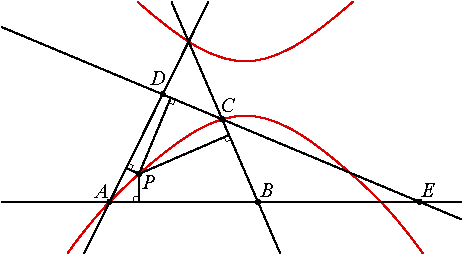
\includegraphics[width=200pt]{main/Pappusproblem}
\caption{The Pappus problem: the product of the distances of $P$ from
the lines $AB$ and $BC$ is proportional to the product of the distances
of $P$ from the lines $CD$ and $DA$.}
\index{Pappus problem}%
\label{figPappusproblem}
\end{figure}

This was to infuriate Newton,
\index{Newton @Newton, Isaac}%
 who showed that Greek methods were
indeed adequate to the original Pappus problem. The background here
is that Newton was also engaged in demolishing Descartes's theory of
planetary motion
\index{planetary motion}%
in favour of his own, which led him into the theory
of conic sections and to pose and solve the problem of finding
the conic (or conics) through $n$ points and tangent to $5-n$
lines, which he did in Book I, Section 5 of his \emph{Principia
Mathematica}.
\label{Newtonconics}

It can be argued that the theory of specifically algebraic curves has its
origin in Descartes's method for finding normals
\index{normal!to an algebraic curve}%
to a curve at a point,
which  involved considering all the circles through the given point and
imposing the condition that the equation for the circle be such that it
passes twice through the given point; this circle has its centre on the
normal to the curve. On the basis of three examples, he claimed that
the method always worked  if the curve had an algebraic equation, and
he described a system of linkages
\index{linkage}%
(sliding rulers) that he said could
be adapted to draw any such curve. Curves like the cycloid
\index{cycloid}%
that were
patently not algebraic he sought to exclude from geometry\emdash this
exclusion was something else that annoyed Newton.

In the 1660s and 1670s, but only published  the 1690s and again in
1704 as an Appendix to his \emph{Opticks}, Newton worked on a
classification of cubic curves.
\index{cubic curve!classification of --s}%
 He claimed that there were 72 distinct
types which could be derived by simplifying the general equation using
what we would call affine or linear transformations, although at one
point he used a simple birational transformation. For some reason, in
writing up his work for publication he omitted four of the possible
cubics, and they were speedily found by various other mathematicians.
Newton also made the striking remark that this collapses to five types
if projective transformations
\index{projective geometry}%
are allowed.%
\footnote{``The five divergent parabolas, by their shadows, generate
  all other curves of the second genus [i.e., cubic curves].'' See
  (Newton  1704) and Talbot (1860, p.~25).}





A plane cubic curve
\index{cubic curve!plane}%
is defined by an equation involving ten coefficients,
or more precisely by the nine ratios between the coefficients, which
suggests that it should be determined by nine points in the plane
because their coordinates provide nine equations that should determine
these nine ratios.  Moreover, it seemed to mathematicians in the early
18th century that any set of nine points and therefore any set of nine
equations in the nine unknowns should have a unique solution\emdash there
was no theory of linear equations at the time\emdash  and as a result even
the best mathematicians got into difficulties. For example, the Scottish
mathematician Colin MacLaurin
\index{MacLaurin, Colin}%
 knew in 1720 that there were problems
with the idea that nine points in the plane should determine a cubic:
any two cubics will meet in nine points, and so these nine points do not
determine a unique cubic, and indeed there will be infinitely many cubics
through these nine points.%
%
\footnote{MacLaurin also knew that a general
cubic curve has nine flexes,
\index{flex}%
and the line joining any two passes through
a third.}  
%
Maclaurin did not, however, know how to solve this puzzle.
This apparent contradiction with the claim that nine points in the plane
always determine a unique cubic became known as Cramer's paradox when
the Swiss mathematician Gabriel Cramer
\index{Cramer @Cramer, Gabriel}%
\index{paradox!Cramer's}%
addressed the problem in his
book (1750, Chapter 3).  Part of the confusion at the time was a lack
of insight into systems of linear equations, and part was the lack of
understanding about what are the implications of configurations that do
not determine a unique curve.


\hskip-1pt
More interestingly, Cramer also suggested that if the $\haa n(n+3)$ points
needed to determine a curve of degree $n$ contain $tn$ points common to
a curve of degree $t < n$ then the curve through the  $\haa (n+1)(n+2)$
points breaks up into two or more curves, one of which passes through
the $tn$ points. We note that Cramer considered only irreducible curves:
a circle and a line, for example, would be considered as two curves,
not one.%
%
\footnote{Curves were taken to be irreducible even in Salmon's
\index{Salmon @Salmon, George}%
book \emph{Higher Plane Curves} (1852).}

Cramer conveyed the (incorrect) claim about cubic curves, and more
generally the analogous claim for curves of degree $n$\emdash  that
they are determined by $\haa n(n+3)$ general points\emdash  to his
friend Leonhard Euler,
\index{Euler @Euler, Leonhard}%
 who repeated  them in the second volume of his
\emph{Introductio} (1748, \S\,81). Euler then wrote a paper (Euler
1750) in which he first spelled out the problem. It is a general
proposition, he said, that $k$ linear equations in $k$ unknowns have
a unique solution. Accordingly, 9 points in the plane will determine a
unique cubic curve. But nine points common to two cubics plainly do not
determine a unique cubic curve.
\index{cubic curve!going through nine points}%
 To resolve this apparent contradiction,
as he called it, he began with  three equations in three unknowns and
showed by example that there will not be a unique solution if one of these
equations is contained in (that is, is a consequence of) the others. He
drew the same conclusion about four 
\index{linear equation, system of --s}%
\index{linear dependence}%
linear equations in four unknowns,
and stated more generally that there will not be a unique solution to
a system of $n$ equations in $n$ unknowns if one or more are contained
in all the others.

He then turned to the geometrical implications. In the case of conics,
he showed that the containment condition corresponds to the case when
four, or all five, of five given points lie on a line.  For cubics,
he remarked that one easily understands that not just one, but two or
more of the nine equations specified by nine points may be contained in
the others, and to obtain a unique cubic it will be necessary to specify
that the curve passes through one or more additional points.  However,
he said, it was very difficult to see what the consequences were when
this is the case, because there were so many points and coefficients
that things become too complicated, although it was possible to draw
conclusions in simple cases. For example, if the nine equations arise in
part from four points lying on a line then the remaining five equations
must determine a conic, which might itself consist of two lines. Euler
concluded his paper with a few remarks about curves of higher degree.


The idea that algebraic curves of degrees $k$ and $m$ in the plane should
meet in $km$ points was something of a folklore result in the early
18th century, but it travelled without a proof for many years. Euler
discussed it in the second volume of his  \emph{Introductio} (1748,
Chapter 19) and noted that even in simple cases  for the counting to
\index{Euler @Euler, Leonhard}%
work one would have to take care of multiple points
\index{multiple point}%
(such as tangents),
points `at infinity'
\index{infinity, line/point at}%
(consider a parabola
\index{parabola}%
and a line parallel to its
axis), and allow the  coordinates of intersection points to be complex
(consider the intersection of two circles). The first person to find
a persuasive way of tackling the problem was \'Etienne B\'ezout,
\index{Bezou@B\'ezout, \'Etienne}%
 who
lived from 1739 to 1783, and made his living teaching mathematics at
the French military and naval academies. He published the theorem that
bears his name in a book of 1779; it is based on his theory of the
resultant
\index{resultant}%
of two polynomial equations that he developed in a paper of
1764. His proof of the theorem is gappy and intuitive by any standards,
but so much better than what had been done before that his immediate
successors were willing to give him real credit for doing as much as he
\index{Cauchy @Cauchy, Augustin-Louis}%
\index{Sylvester @Sylvester, James Joseph}%
did. His results inspired later work by Cauchy and James Joseph Sylvester.

To state  B\'ezout's theorem in general requires a notion of the
multiplicity
\index{multiplicity!of an intersection}%
of an intersection of two plane curves without common
components. Such a notion was developed by Max Noether,
\vadjust{\goodbreak}%
\index{Noether @Noether, Max}%
 and refined
\index{Macaulay @Macaulay, Francis Sowerby}%
by Francis Sowerby Macaulay.
 A modern proof would invoke Noether's
Fundamental Theorem\emdash see p.~\pageref{Noether'sFT}\emdash and a
computation of the Hilbert polynomial.
\index{Hilbert polynomial}%
\index{fundamental theorem!(Noether)}%
 This is a story that  has been
pursued, with successive new generalisations, right up to the present day.


As this activity suggests, throughout the 18th century mathematicians
had become more and more comfortable with the idea of complex numbers in
algebra, and with the idea of proving that a polynomial of degree $n$ has
$n$ roots, possibly with repetitions (the so-called fundamental theorem
of
\index{fundamental theorem!of algebra}%
algebra).%
%
\footnote{For a history of attempts on this theorem, see (Gilain 1991).} 
%
Euler's attitude to complex numbers was that there was
\index{Euler @Euler, Leonhard}%
nothing to explain. Although they cannot be ordered, expressions of the
form $a+bi$  behave arithmetically like numbers, so they can reasonably be
\index{imaginary numbers, naming of}%
considered numbers  and ``are usually called \emph{imaginary quantities},
because they exist merely in the imagination.''%
\footnote{See Euler,
\emph{Algebra} \S\,143, p.~43. Euler here rejected the idea that
ultimately mathematical quantities must be exhibited in nature: three
sheep, a length of $\sqrt{2}$, and so on.}
%
Cauchy's view later was more
explicit and very close to regarding  the field of complex numbers as
$\RR [x]/(x^2 + 1)$. This works for finding a proof of the fundamental
theorem of algebra, which he gave a proof of in his (1817a, b), but was
not productive in contexts involving contour integration.
\index{contour integration}%


Credit for the first rigorous proof of the fundamental theorem is often
given to Carl Friedrich Gauss
\index{Gauss @Gauss, Carl Friedrich}%
for his paper (1799), although he did
base his argument on the claim that an algebraic curve that enters a
bounded region of the plane also leaves it,  which is surely no easier
to prove.  Gauss went on to give three more proofs of the theorem,
and soon any doubts about the algebraic nature of complex numbers were
resolved.%
%
\footnote{William Rowan Hamilton
\index{Hamilton @Hamilton, William Rowan}%
published his rigorous theory
of ordered pairs of real numbers in his (1837).}
%
Niels Abel
\index{Abel @Abel, Niels}%
and Carl Gustav Jacob Jacobi,
\index{Jacobi @Jacobi, Carl Gustav Jacob}%
 in their work  on elliptic functions, took a formal,
non-geometrical attitude to complex numbers.  Both men were algebraists
at heart\emdash formidable algebraists\emdash and the exact nature the
plane of complex numbers did not really interest them.

All things considered, however, progress in the study of cubic, quartic,
\index{cubic curve}%
\index{quartic curve}%
and higher degree curves in the 18th century was piecemeal and slight, and
the sheer enormity of the equations involved seems to have baffled even
Euler. New methods for handling such curves would have to be found, such
as came in with Pl\"ucker
\index{Pl\"ucker, Julius}%
in the 1820s. His key idea was to study families
of curves, using the symbolic notation devised by Gergonne.%
%
\footnote{See (Gergonne 1826--1827), (Pl\"ucker 1835) and (Pl\"ucker 1839).} 
%
If $S_1$
and $S_2$ stand for the equations of two curves of the same degree,
\index{pencil!of curves}%
then $S_1 + \lambda S_2$ is generally the equation of another curve of
that degree. This may be the first occurrence of the idea of a linear
series,
\index{linear series}%
 with which this book is much concerned. Using this idea allowed
Pl\"ucker to pull out geometrical properties of cubic and quartic plane
curves while avoiding the algebraic complexities that had defeated Euler.

Pl\"ucker also resolved the paradox
\index{paradox!about dual curves}%
\index{duality!paradox}%
about dual curves in the theory of
plane curves in his (1834) that had stumped Gergonne
\index{Gergonne @Gergonne, Joseph Diaz}%
and Poncelet.
\index{Poncelet @Poncelet, Jean Victor}%
 The
paradox arises because the dual
\index{dual curve}%
of a smooth curve of degree $d$ has
degree $d(d-1)$
so the dual of the dual ``ought'' to have degree
$d(d-1)(d(d-1)-1)$. However, the dual of the dual is the original curve.
Pl\"ucker's response, which would strike us today as at best heuristic,
was that any line through a double point, say, is counted in this way
as a tangent, and this throws the count of genuine tangents off. More
precisely, he  showed that each node
\index{node}%
on a curve reduces the degree
of the dual curve by 2, and each cusp
\index{cusp}%
reduces it by 3. Consequently,
he claimed that  a curve of degree $d$ with $\delta$ double points and
$\kappa$ cusps has a dual curve  of degree $d(d-1) -  2\delta - 3\kappa$.




Pl\"ucker also showed in his (1839, 207--227) that the nodes of $C^{*}$,
the dual curve of $C$,  corresponded to the bitangents
\index{bitangent}%
of $C$, while
the cusps of $C^{*}$ corresponded to the flexes
\index{flex}%
of $C$, and vice
versa. To see how he resolved the duality paradox, consider  the case
of a non-singular cubic curve. It has no nodes, cusps, or bitangents,
and an as yet indeterminate number, $j$ of flexes. Its dual has degree 6
and $j$ cusps. The dual of the dual curve therefore has degree $6\cdot 5 - 3j$,
\index{MacLaurin, Colin}%
which will equal 3 if $j = 9$. As we saw, the result that a non-degenerate
cubic curve has nine flexes had been known since MacLaurin. For curves of
higher degree, it is necessary to consider a curve of degree $n$ that has
$\delta$ double points, $\kappa$ cusps, $\tau$ bitangents, and $\iota$
inflections. Suppose that its dual has degree $n'$. Pl\"ucker argued that
$$
n' = n(n-1) - 2\delta - 3 \kappa
\quad
\hbox{and}\quad \iota = 3n(n-2) - 6\delta - 8\kappa,
$$
with another formula for $\tau$, along with the corresponding formula
for the dual curve and its inflection points and bitangents.

The number $\iota$ is most easily found using an argument due to
Ludwig Otto Hesse,
\index{Hesse @Hesse, Ludwig Otto}%
 who showed  in his (1844)  that the set of flexes
$\Gamma\subset G$ on a curve $G$ of degree $d$ with equation $F(x, y, z)
= 0$ could be characterized as the intersection of $G$  with the curve
$D$ defined by the vanishing of the \emph{Hessian determinant}:
\index{Hessian}%
$$
H = \det \begin{pmatrix}
 \partial^{2}F/\partial x^{2} &\partial^{2}F/\partial x\partial y
 &\partial^{2}F/\partial x\partial z \\
\partial^{2}F/\partial x\partial y  &\partial^{2}F/\partial y^{2}
&\partial^{2}F/\partial y\partial z \\
\partial^{2}F/\partial x\partial z &\partial^{2}F/\partial y\partial z
&\partial^{2}F/\partial z^{2}
\end{pmatrix}.
$$
Since the entries of this matrix have degree $n-2$, the degree of $H$
is $3(n-2)$. For general $F$ the curves $G$ and $D$ meet transversely, so
B\'ezout's Theorem
\index{Bezout@B\'ezout's theorem}%
shows that a general curve of degree $m$ has exactly
$\iota = 3n(n-2)$ flexes.%
%
\footnote{This result was first proved in a
different way in (Pl\"ucker 1835, 264), as Hesse acknowledged.}

The most famous case Pl\"ucker
\index{Pl\"ucker, Julius}%
established in  his book (1839, 247),
concerns   a nonsingular plane curve $C$ of degree $n=4$  (no nodes,
cusps, or other singular points) having $\tau$ bitangents
\index{bitangent}%
and $\iota$
flexes.
\index{flex}%
Its dual curve has degree 12 and will have $\tau$ double points
and $\iota$ cusps, and the dual of the dual will have degree
$12\cdot 11 - 2\tau - 3h  = 4$.
Hesse's theorem shows that $h = 24$ (Pl\"ucker  had an ad hoc argument to
the same effect)  and so $\tau = 28$,  and we  see that $C$ has exactly
28 bitangents. Pl\"ucker showed that they can all be real (see Figure
\ref{fig28bitangents}).

In 1849, Pl\"ucker gave up mathematics for physics, particularly the study
of cathode rays; he was awarded the Royal Society of London's Copley
medal
\index{Copley medal}%
(its highest honour) for this work in 1866. It is sometimes said
that he gave up geometry because he tired of the criticisms of Steiner,
\index{Steiner @Steiner, Jakob}%
who had a secure position in Berlin and influenced the decisions of the
\index{Journal@{\it Journal f\"ur die reine und angewandte Mathematik}}%
\emph{Journal f\"ur Mathematik}, and only returned to geometry after
Steiner died in 1863. Now he took up  the field of line geometry,
\index{line geometry}%
 which
he transformed into a new branch of the subject.

\begin{figure}
\fboxsep0pt
\fbox{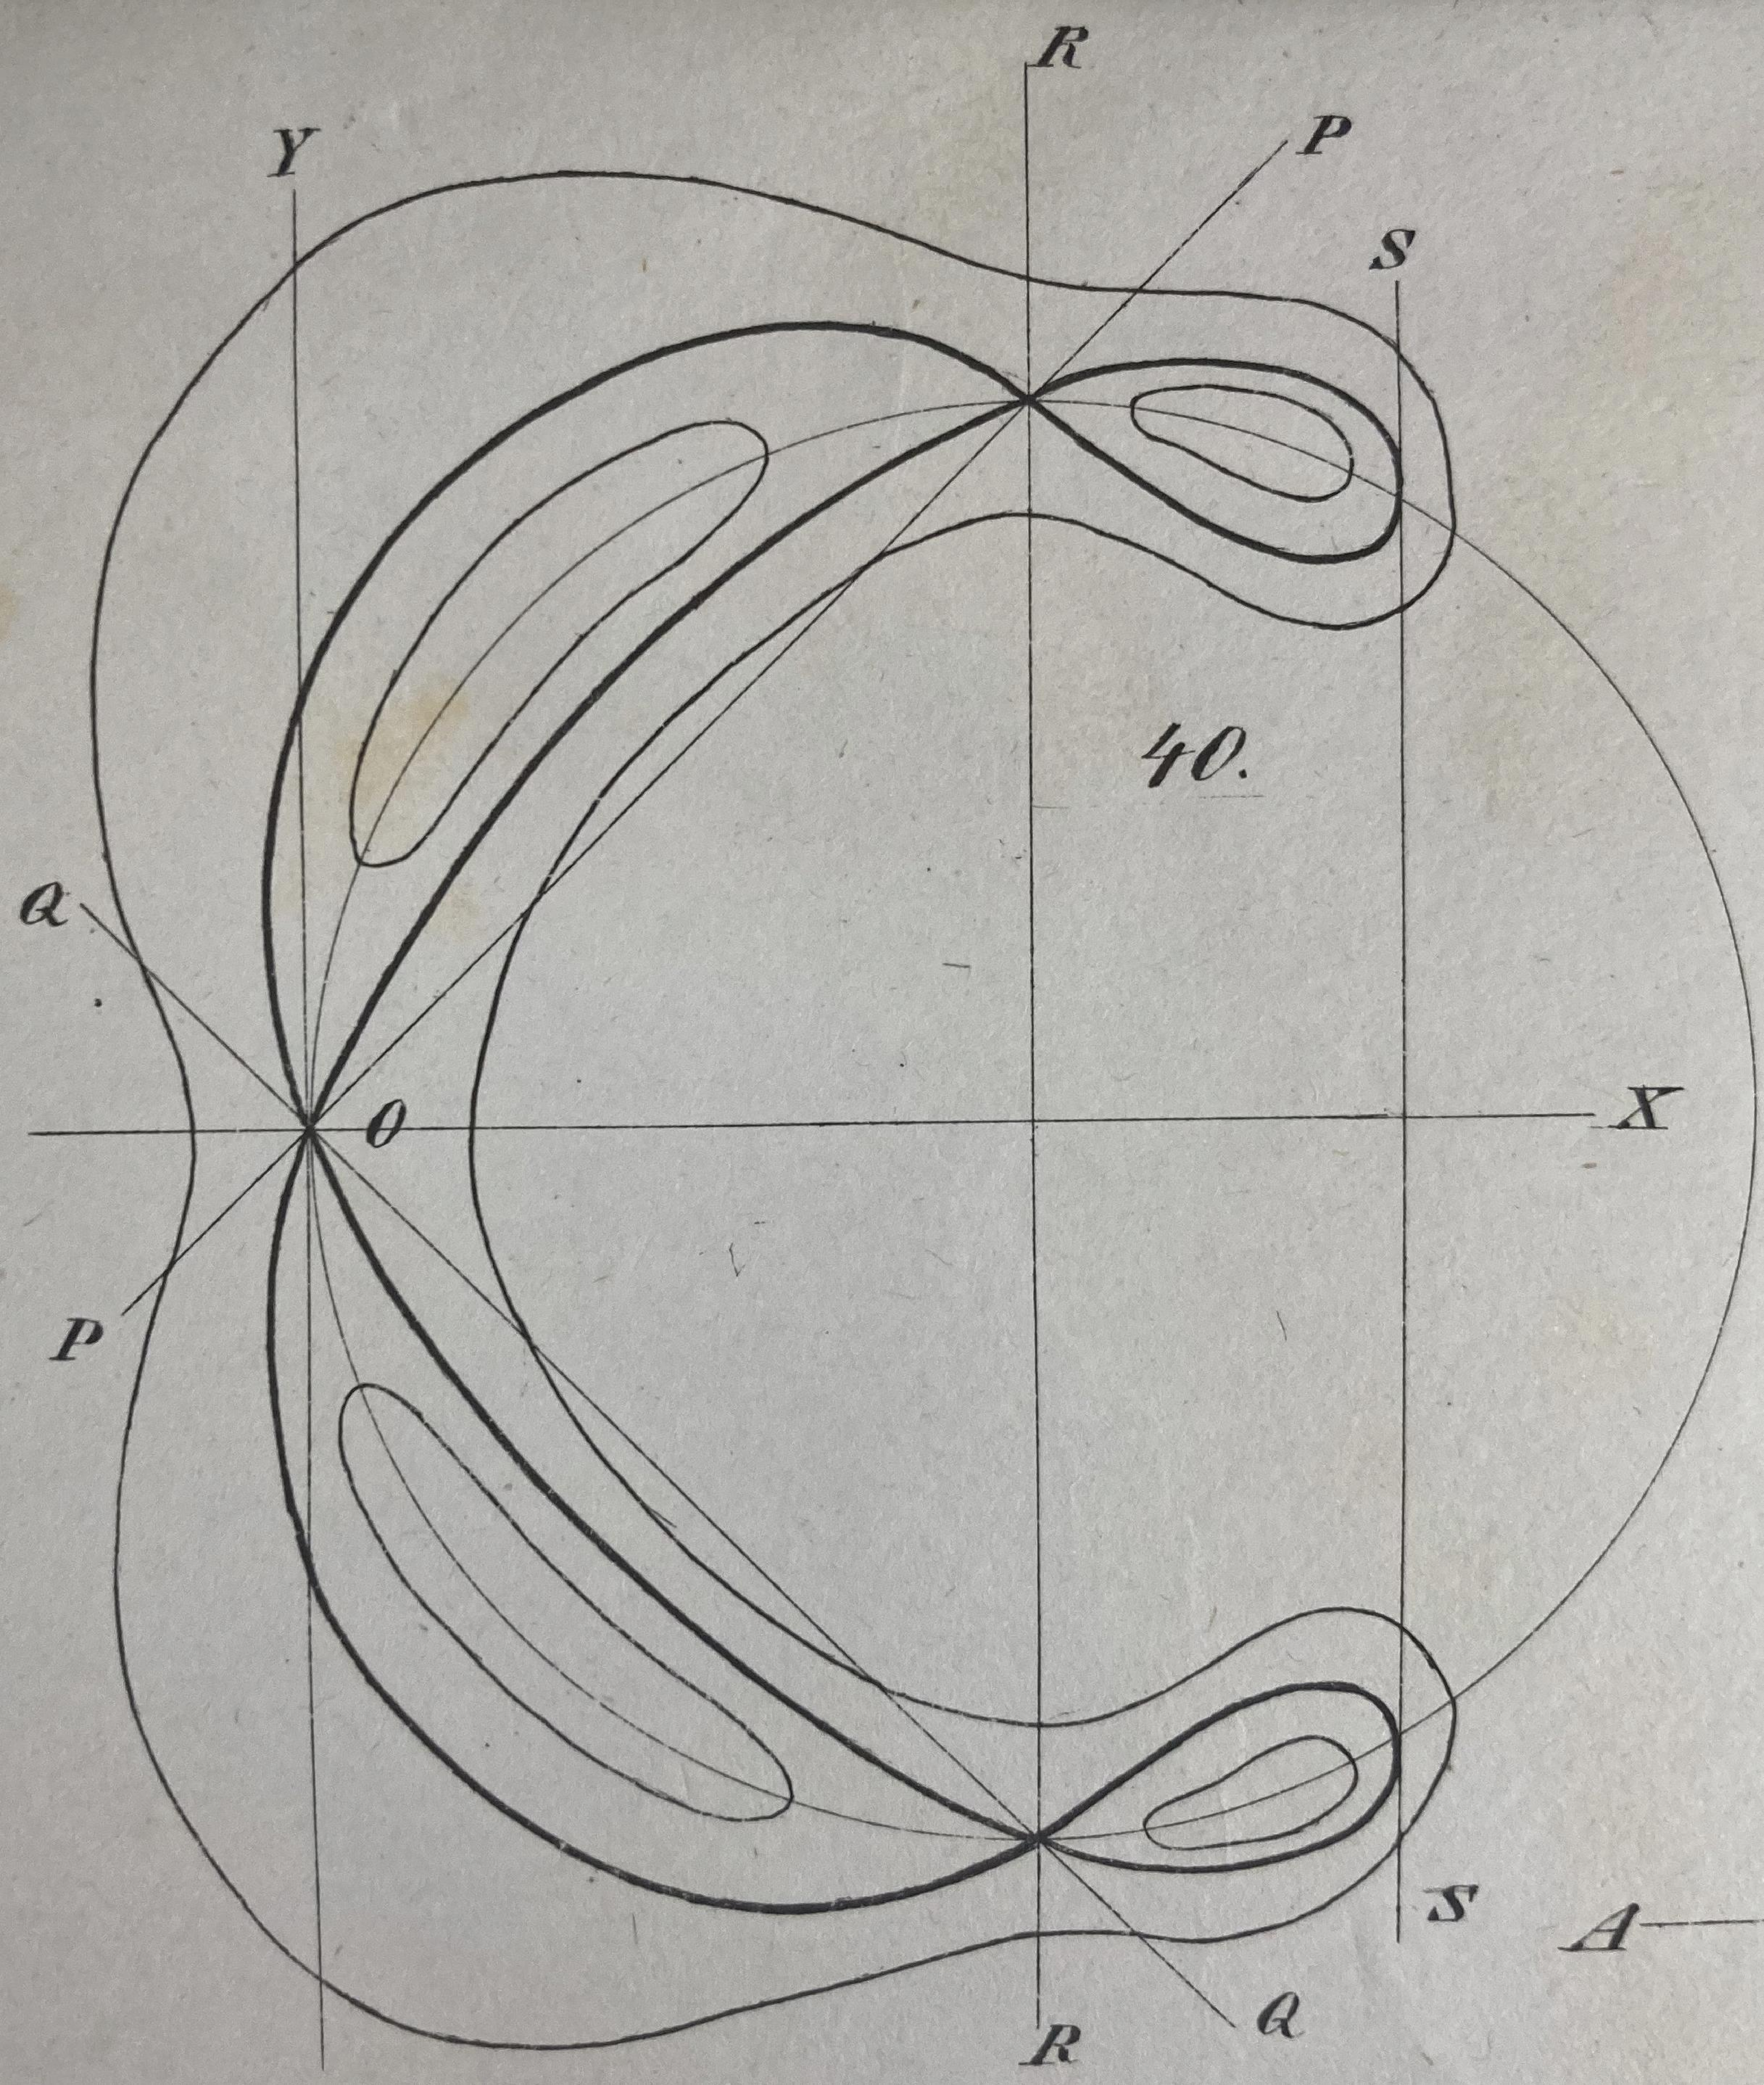
\includegraphics[width=15em]{main/Gray-scan-Fig2-cropped}}
\caption{Pl\"ucker's quartic curve has 28 bitangents. From (Pl\"ucker
1839).}
      \label{fig28bitangents}
\end{figure}

Pl\"ucker's formulae work well for curves of degrees 3 and 4,  but not so
well thereafter because other types of singularity
\index{singularity!higher}%
can appear.   He listed
all the solutions he could find to the equations that bear his name up to
curves of degree 10, but he did not discuss the kinds of singularities a
curve may have that are not of the type he had considered.%
%
\footnote{See (Pl\"ucker 1839, 214).}  
%
Progress was only made with a paper by Arthur
Cayley
\index{Cayley @Cayley, Arthur}%
(1866), who drew on Victor Puiseux's
\index{Puiseux @Puiseux, Victor}%
paper (1850) that analysed
how curves are ramified at a singular point,  showed how the branches are
\index{ramification}%
permuted in cycles, and how this is captured by the local power series
\index{power series}%
expansions, which begin with fractional indices.%
\index{fractional exponent}%
%
\footnote{Cayley's paper
was corrected by Otto Stolz
\index{Stolz @Stolz, Otto}%
in his (1875), who found that the conclusions
were correct but the proof ``as he [Cayley] himself remarks'', was not
quite complete.}

Puiseux was one of a number of mathematicians in the circle around
\index{Cauchy @Cauchy, Augustin-Louis}%
Cau\-chy. Cauchy had spent the 1830s and early 1840s following the
Bourbon Court around Europe from a strange belief that the oath of
allegiance he had sworn to the crown on becoming a professor compelled
him to do so. As a result, by 1850 few people knew the work he had done
in those years, and even he seems to have forgotten what he had done
in complex variable theory back in the 1820s, which included a version
of what we call the Cauchy integral theorem
\index{integral theorem (Cauchy)}%
\index{Cauchy integral theorem}%
(Cauchy 1825) restricted
to rectangular contours. Only on his return to Paris did he begin to
think much more geometrically; previously his attitude to a many-valued
`function' was to cut the plane and study just a branch of it on what
remains. His understanding of branch points was quite limited, and this
left space for Puiseux to study integrals on arbitrary contours   and
what happens to integrals taken around branch points.

\section{The birth of projective space}
When did projective space
\index{projective space}%
come to be regarded as something more rigorous
than Euclidean space with a ``line at infinity''?%
%
\footnote{For an
interesting  set of essays analysing what projective space might be and
how it came about, including an extensive analysis by J.-P.
Friedelmeyer
\index{Friedelmeyer, Jean-Pierre}%
of the work of Poncelet, see (Biosemat-Martagon 2010), and the discussion
\index{Centina@del Centina, Andrea}%
in del Centina's \emph{The History of Projective Geometry} (to appear).}
%
 This might simply be a suitable set of coordinates. Pl\"ucker used
 coordinates for the plane with a line at infinity in his (1830) with
 a view to enabling homogeneous equations
\index{homogeneous equation}%
to correspond to curves; in
 this system the coordinates $(p, q, r)$ denote the signed distances of
 a point from the three sides of a triangle of reference. However, in
 his study of curves (1835) he would first discuss them in  the plane,
 and then as they went off to infinity; he didn't say that the line at
 infinity could be mapped by a projective transformation into the finite
 part of the plane.  The way forward was indicated by August M\"obius,
\index{M\"obius, August}%
 who introduced barycentric coordinates
\index{barycentric coordinates}%
in his (1827). Pick three points
 forming a triangle, say $ABC$, and attach weights, positive, zero, or
 negative (not all zero) to these points. The barycentre or centre of
 gravity of these three weighted points is a point $P$ which can be said
 to have those three weights (or, better, their ratios) as its barycentric
 coordinates. If you put the points $A, B, C$ at, say,  $(0, 0), (1, 0),
 (0, 1)$ you get an easy way to relate points in what could be called
 the Cartesian and barycentric coordinate planes. The big plus is that
 the line at infinity,
\index{infinity, line/point at}%
 which is invisible in Cartesian coordinates, is
 a perfectly sensible line in barycentric coordinates. In this system,
 a line has an equation of the form $ax+by+cz=0$, and by treating $a,
 b, c$ as the coordinates of the line M\"obius obtained a simple theory
 of conics and duality in the plane. (He also showed that there are
 dualities in $P^3$ that are not pole-polar dualities.)

If you drop the talk about weights, and keep the idea that barycentric
coordinates are best thought of as ratios of three numbers, you have
projective coordinates;
\index{projective coordinates}%
 this was one of the contributions of Hesse in
\index{Hesse @Hesse, Ludwig Otto}%
the 1840s.%
%
\footnote{See, for example, (Hesse 1844).}
%
Mathematicians were still reluctant, however, to decide if this space
\index{projective space!complex}%
was $\PP_{\RR}^2$ or, less likely, $\PP_{\CC}^2$.

Mathematicians found it hard to accept complex coordinates, even
though Pl\"ucker used the term `imaginary' (as in `imaginary' points,
`imaginary' straight lines, `imaginary' tangents) over two hundred
times in his (1828--1831).%
%
\footnote{Del Centina, \emph{The History of Projective Geometry},
\index{Centina@del Centina, Andrea}%
forthcoming.}
%
He employed the term
confidently in his (1839) when, for example, he discussed how many of
the 28 bitangents to a quartic curve can be real. In fact, the whole
question of a complex space was obscure for a long time. As late as
1878 Cayley
\index{Cayley @Cayley, Arthur}%
could write about complex curves as sets of points in
$\CC \times \CC$ and remark ``I was under the impression that the
theory was a known one; but I have not found it set out anywhere in
detail.''%
%
\footnote{See (Cayley 1878, 32).} 
%
For quite some time
attention was fixed on real curves in the real plane, which could
conveniently sprout points with complex coordinates when they
intersected other curves. This unstable situation could not last, but
how it was to be swept away was not clear to mathematicians initially.


\section{Riemann's theory of algebraic curves and its reception}
It was, however, entirely clear to Riemann. The crucial issue in defining
com\-plex-valued functions of a complex variable, where a complex
variable
\index{complex functions}%
can be taken as an expression of the form $x+ iy$, is defining what it is
for such a function to be something more particular than a mapping from
$\RR^2$ to $\RR^2$, and this comes down to defining what it is for such
a function to be differentiable as a function of a complex variable. As
is well-known, Riemann
\index{Riemann @Riemann, Georg Friedrich Bernhard}%
\index{Cauchy @Cauchy, Augustin-Louis}%
solved this problem in the opening pages of
his inaugural dissertation  (1851) by identifying\emdash much more
clearly than Cauchy\emdash the role of what we call the Cauchy--Riemann
equations. He proceeded to give a thoroughly geometric theory of complex
functions, which he extended in his great paper on Abelian functions
\index{abelian function}%
(1857). There he developed a strikingly topological account, which
classified orientable, boundaryless surfaces by the number, $2p+1$,
of cuts needs to disconnect them. He called this number the order of
connectivity of the surface, when $p=0$ he called the surface simply
connected. The theory is too complicated to be described fully here,
but briefly, he showed that  the dimension of the space of ``everywhere
finite'' differential forms
\index{differential form}%
on such a surface is $p$, and the integral
of each such
differential gives rise to a many-valued function, which can be expressed
in the form $f(z, w) = 0$, where $z$ and $w$ are complex variables. He
also deduced the Riemann inequality
\index{Riemann inequality}%
in this form (1857, \S\,5):  the
number of arbitrary constants in a function $w$ that has $m$ first-order
poles on a surface of order of connectivity $2p+1$ is $m- p + 1$ when $m
\geq p + 1$. He gave a more detailed account that involves special cases
\index{Roch @Roch, Gustav}%
that were interpreted by his student Roch to give us the Riemann--Roch
theorem.
\index{Riemann--Roch theorem}%

Riemann's health started to decline in the early 1860s, and he  died
in Italy in July 1866. By then, Rudolf Clebsch had
\index{Clebsch @Clebsch, Rudolf Friedrich Alfred}%
decided to develop
Riemann's ideas and to try to persuade people around him to take up the
cause. In his (1864) he  applied the theory of Abelian functions to the
study of plane algebraic curves. Here he used coordinates that belonged
either to $\CC^2$ or $\PP_{\CC}^2$ and  passed easily between them as
required, so it would seem that he and the people he influenced had
become comfortable with complex projective space in all but name.

In his papers (1865a, 43) and (1865b, 98) Clebsch sorted curves into
\index{genus}%
different genera according to the value of the number $p$ associated
to them, but he did not speak of the genus of a curve.%
%
\footnote{See
(L\^e 2020), who suggests that Felix Klein
\index{Klein @Klein, Felix}%
was the first to do so.} 
%
If
we allow ourselves to do so, we may say that Clebsch defined the genus
of a plane algebraic curve with $\delta$ double points as%
%
\footnote{See (Clebsch 1864, 192).}
%
$$p = \haa (n-1)(n-2) - \delta.$$
In his (1865b) and his book with Paul Gordan
\index{Gordan @Gordan, Paul}%
(1866) he extended this to
encompass curves with
$\kappa$ cusps,
\index{cusp}%
 so $p= \haa (n-1)(n-2) - \delta - \kappa$. This tells
us incidentally that no singular points more complicated than those
considered by Pl\"ucker in the late 1830s had been looked at. Clebsch's
\index{singularity!higher}%
formula relied on being able to count the number of constants in an
integral of an everywhere finite differential correctly, a result that
requires the  completeness of the adjoint series. Clebsch and Gordan offered
in their book (1866, Chapter 3) a proof that the genus of a plane
algebraic curve is invariant under a birational transformation,
\index{birational!transformation}%
 but it was
valid only for the case of a curve with simple cusps and double points.
\index{cusp}%

Clebsch became   Riemann's successor in G\"ottingen
\index{Gottingen@G\"ottingen University}%
in 1868, but  he
died of diphtheria in 1872 at the age of 39. His plans for the study of
algebraic geometry now devolved upon Alexander Brill
\index{Brill @Brill, Alexander}%
and Max Noether,
\index{Noether @Noether, Max}%
with whose theory, modernised and made rigorous,  this book is in part
concerned.%
%
\footnote{A modern account of  much of the material described
above can be found in (Brieskorn and Kn\"orrer 1986). (Coolidge 1940)
remains a historically informative if not entirely rigorous account of
many of these developments, more additional mathematical details are in
(Coolidge 1931).}

Alexander Wilhelm Brill was born in Darmstadt in 1842.%
%
\footnote{See
(Severi 1922),  and Brill's obituary (Finsterwalder 1936).}
%
His  uncle was
the mathematician Christian Wiener,
\index{Wiener @Wiener, Christian}%
 an expert in descriptive geometry.
\index{descriptive geometry}%
 He
entered the University of Giessen
\index{Giessen University}%
intending to study architecture but his
mathematical ability brought him to the attention of Clebsch, who was then
at Giessen and who encouraged him to go  to Berlin, where  Ernst
Kummer,
\index{Kummer @Kummer, Ernst}%
Leopold Kronecker,
\index{Kronecker @Kronecker, Leopold}%
 and Karl Weierstrass
\index{Weierstrass @Weierstrass, Karl}%
taught. This broadened Brill's
horizons considerably, but he returned to Giessen in 1867 to take his
\index{Clebsch @Clebsch, Rudolf Friedrich Alfred}%
Habilitation  under Clebsch.

In Giessen, Brill met Max Noether.
\index{Noether @Noether, Max}%
 Noether had been born in Mannheim
in 1844, but polio at the age of 14 left him paralysed in one leg and
delayed his education. He had to be privately schooled, which gave
him  broad literary and cultural interests. At university he  initially
intended to study astronomy, but then he switched to mathematics, first
at Heidelberg
\index{Heidelberg University}%
and then at Giessen and G\"ottingen
\index{Gottingen@G\"ottingen University}%
in 1868 and 1869. He
habilitated in Heidelberg in 1870 with a thesis on surfaces possessing
a family of rational curves. In 1875 he became a Professor at Erlangen,
\index{Erlangen University}%
where he remained until his death in 1921.%
%
\footnote{See his obituary
(Brill 1923).}


Noether  worked not only on plane algebraic curves, including the analysis
of their singular points, but the geometry of algebraic surfaces,
algebraic curves in space, and Cremona transformations
\index{Cremona transformation}%
of the plane;
van der Waerden justly remarked that ``Algebraic geometry
\index{algebraic geometry, founding of}%
was created by
Max Noether.''%
%
\footnote{See (Waerden 1971, 171) who immediately commented
that the logical foundations are shaky.}
%
He drew largely on the work of Pl\"ucker
\index{Pl\"ucker, Julius}%
on algebraic curves and their
singular points, and was less interested in the computational side of the
theory that Clebsch had emphasised. As a result, his obituarists\emdash
Guido Castelnuovo,
\index{Castelnuovo @Castelnuovo, Guido}%
 Federigo Enriques,
\index{Enriques @Enriques, Federigo}%
 and Francesco Severi\emdash
\index{Severi @Severi, Francesco}%
noted
that Noether's work was inclined to be qualitatively valuable even though
he may not have paid sufficient attention to ``contingent aspects of
the formulae''.  However, they added that:%
%
\footnote{See (Castelnuovo,
Enriques, and Severi 1925, 162)}
%
\begin{quote}
geometric intuition, which was always his guide, saved him from error,
and the work, even if it was not perfect, and perhaps for that reason,
was richly suggestive.
\end{quote}



Brill  chafed under the direction of  Richard Baltzer, who
\index{Baltzer @Baltzer, Richard}%
was Clebsch's
\index{Clebsch @Clebsch, Rudolf Friedrich Alfred}%
successor at Giessen,  and moved to the new Polytechnic in Darmstadt
\index{Giessen University}%
\index{Darmstadt Polytechnic}%
in 1869, which was academically a step downwards. There, he did his
work on the Cayley--Brill correspondence principle, and in 1875  he
accepted Klein's offer of becoming a Professor at the Polytechnic
\index{Munich Polytechnic}%
in Munich, with responsibility for reforming high school education.
Brill found Klein's inventiveness
\index{Klein @Klein, Felix}%
hard to match, but he enjoyed getting
to know some of the other mathematicians there, including Philipp
Seidel
\index{Seidel @Seidel, Philipp}%
and the young Alfred Pringsheim. Among
\index{Pringsheim @Pringsheim, Alfred}%
his pupils were Walther Dyck,
Isaak
\index{Dyck @Dyck, Walther}%
\index{Bacharach @Bacharach, Isaak}%
Bacharach, and Ferdinand Lindemann,
\index{Lindemann @Lindemann, Ferdinand}%
 who went on to produce the
two-volume geometry textbook \emph{Vorlesungen \"uber Geometrie} (known
as Clebsch--Lindemann) before achieving fame as the mathematician who
proved that $\pi$ is transcendental.
\index{pi@$\pi$ transcendentality}%
\index{transcendentality of $\pi$}%


\section{First ideas about the resolution of singular points}
In their work on algebraic curves, Brill and Noether found Riemann's use
of the Dirichlet principle
\index{Dirichlet principle}%
at the heart of his theory of complex analytic
functions
\index{complex functions}%
to be unsound, so they studied curves firmly in the complex
plane $\CC^2$ or the complex projective plane $\PP_{\CC}^2$. They were
concerned to treat such curves in full generality, and this led them
to confront the issue of arbitrary 
singularities
\index{singularity!higher}%
of plane curves. Their
preferred method was to argue that any curve with whatever singularities
could be reduced to one of the same genus but having only double points
by a sequence of Cremona transformations,
\index{Cremona transformation}%
 and then to deal in detail
with these simpler curves. It was clear from the formula for the genus
\index{genus}%
of a plane curve that if the genus of the curve is not a triangular
number then the curve will always have singular points, so the process
of desingularising cannot always lead to a nonsingular curve.

Luigi Cremona
\index{Cremona @Cremona, Luigi}%
had  outlined a general theory of transformations of
the plane in his papers (1863) and (1865). He looked for geometrical
transformations of the plane mapping a given figure one-to-one onto its
image, and reciprocally; notably  transformations that map straight lines
to curves of order $n$, for some $n$. When $n=2$ (the case of quadratic
transformations)  as he showed, almost all straight lines must have
images that are conics passing through 3 fixed points.%
%
\footnote{Such
examples had been studied before; Cremona  cited papers by Steiner,
\index{Steiner @Steiner, Jakob}%
\index{Magnus @Magnus, Leopold}%
Magnus, and Schiaparelli,
\index{Schiaparelli @Schiaparelli, Giovanni Virginio}%
 but for higher values of $n$, which Cremona
analysed in his (1865), everything was new.}



Noether in his (1871a) was the first to appreciate that Cremona
transformations could be used to simplify singular points.  He wrote a
Cremona transformation of the plane algebraically as
$$
[x,y,z] \mapsto [x',y',z'] = [\phi (x,y,z), \psi (x, y, z),  \chi (x,
y, z)],
$$
where the functions $\phi, \psi$ and $\chi$ are homogeneous polynomials
in $x, y$ and $z$ of the same degree. To simplify a singular point he used
transformations defined as above where $\phi, \psi$, and $\chi$ all
vanish at the singular point.  In the affine plane this becomes
$$(x , y) \mapsto (x_1 , y_1) = \left(\frac{\varphi (x, y)}{\chi (x,
y)}\,,  \frac{\psi (x, y)}{\chi (x, y)} \right),$$
where $\varphi$, $\psi$, and $\chi$ are polynomial functions that vanish
at the singular point.  To see what this does, it is convenient to take
the familiar example of
the simplest  Cremona transformation,
\index{quadratic transformation}%
 other than a projective
transformation. It  is given algebraically by  the quadratic
transformation
\begin{equation*}
[x, y, z] \mapsto \left[\frac{1}{x}, \frac{1}{y}, \frac{1}{z}\right] =
[yz, zx, xy]
.
\end{equation*}
The union of the lines $x=0,y=0,z=0$ is called the exceptional triangle,
and the images of these lines are the points $[1, 0, 0], [0, 1, 0]$
and $[0, 0, 1]$ respectively.
The transformation is many-valued at these points, each of which is
\index{blowup}%
``blown up'' into a line  but it is well-defined away from those three
points and it is  one-to-one away from  the lines $x=0$, $y=0$, and $z
= 0$.


Noether's
\index{Noether @Noether, Max}%
argument that any plane algebraic curve can be reduced to one
with only double points is sketchy at best. His use of Puiseux's
\index{Puiseux @Puiseux, Victor}%
work
suggests that he appreciated that quadratic transformation might have to
\index{desingularization}%
be used repeatedly to reduce a complicated singularity to a simpler one,
but he did not  fully appreciate what happens to the rest of the curve at
the points where it crosses the exceptional lines. In his more rigorous
account  (1876),  he gave a better definition of a singular point, and
\index{genus!invariance under birational maps}%
tried to redefine the genus of a plane algebraic curve and prove its
invariance  under birational  transformations.%
%
\footnote{Noether also
claimed  the remarkable theorem that every such Cremona transformation
is a composition of quadratic transformations and projective
transformations. See his (1871b), with a small correction in his (1873).}


\section{The work of Brill and Noether}
Noether began, in his (1873), with the question of when  a plane curve
$E$ with equation $H=0$ can be expressed in the form $H = AF+BG$,
where $F=0$ and $G=0$ are the equations of two curves $C$ and $D$.
He rightly pointed out that people hitherto had assumed that it was
necessary and sufficient that the curve $E$  passes simply through
the intersection points of the curves $C$ and $D$, but in fact this
is insufficient when the curves $C$ and $D$ have singular points or
intersections with multiple tangents. His own account, which was based
on counting the number of independent equations imposed on $H=0$ by
the equations $F=0$ and $G=0$, was a significant advance, but it too
had flaws and he and other authors, notably Eugenio Bertini, offered
\index{Bertini @Bertini, Eugenio}%
improvements. Eventually, Noether  offered this formulation of his
\index{fundamental theorem!(Noether)}%
Fundamental Theorem\label{Noether'sFT}:%
%
\footnote{See (Noether 1887, 413).}

\begin{untheorem}
%\label{NFT1887}
$H(x, y)$ is representable in the form $AF + BG$ if and only if in some
neighbourhood of each common point $(x_0, y_0)$ of $F=0$ and $G=0$
there are power series $a(x-x_0)$ and $b(x-x_0)$ in $\CC[y]\[x\]$
whose coefficients are polynomials in $y$ of orders  $n-1$ and $m-1$
respectively, such that $H = aF + bG$.
\end{untheorem}

Only in the monumental joint work with Brill
\index{Brill @Brill, Alexander}%
(Brill and Noether 1894,
352) was it shown that in the plane case there is nothing more to be said,
the local conditions are indeed sufficient even in the projective case.


Today we would say that Noether's Fundamental Theorem is true for two
polynomials $F$ and $G$ because $F,G$ is a regular sequence  and so  the
ideal they generate is, in later terminology due to Macaulay (1916),
\index{unmixed ideal}%
\index{Macaulay @Macaulay, Francis Sowerby}%
unmixed.%
%
\footnote{See (Eisenbud and Gray 2023) and (Eisenbud and Gray
2024) for a historical account of Macaulay's work.}

Brill and Noether recognised that the Riemann--Roch theorem was of
\index{Riemann--Roch theorem}%
central importance to the theory of plane algebraic curves; indeed, they
were the first to name it.%
%
\footnote{See (Brill and Noether 1874, \S\,5).}
%
Clebsch had studied what we would call holomorphic diff\-erential forms
\index{holomorphic differential}%
on a curve $C$  of degree $d$ in his (1864, 193)  by supposing that they
are given by homogeneous polynomials of degree $d-3$ that vanish at the
double points of the curve.
By B\'ezout's Theorem,
\index{Bezout@B\'ezout's theorem}%
 such an intersection also has degree $d(d-3) =
2p-2$, as it should. The dimension of the family of divisors cut out
on $C$ in this way is the dimension of the projective space of forms
of degree $d-3$ in $\CC[x_0,x_1,x_2]$, which is conveniently equal to
$(d-1)(d-2)/2$. For this to be correct and account for all the canonical
divisors, it has to be shown that every divisor $E$ on the curve $C$ that
differs from an intersection $D\cap C$, where $D$ is the curve defined
by the equation $G = 0$,  by the divisor of the restriction to $C$ of
a rational function $P/Q$ (where $P, Q$ are forms of the same degree),
is again of the form $D'\cap C$ for some curve $D'$. This is the content
of Noether's Fundamental Theorem. His Fundamental Theorem is essential
\index{fundamental theorem!(Noether)}%
when it comes  to handling  sets of points cut out on a fixed curve $C$ by
families of curves, counting the degree of an intersection of two curves
at multiple points,  dividing an arbitrary intersection into two subsets,
and delivering a satisfactory version of the Riemann--Roch theorem.
\index{historical context|)}%

For reasons of space, it is impossible to pursue the history of curves
after the Riemann--Roch theorem here, except to note that some of the
consequences are the subject of the present book to which this essay
is appended.


\section{Historical bibliography}

\frenchspacing
\def\newline{\par\hangindent=10pt\hangafter=1}
\parindent=0pt % disturbs this file less than erasing all the \indents below
\small
\newline
\indent Anglade, M. and J.-Y. Briend 2022. Nombrils, bruslans, autrement foyerz; la g\'eom\'etrie en action dans le \emph{Brouillon project} de Girard Desargues, \emph{Archive for History of Exact Sciences}, 76, 173--206.
\newline\indent B\'ezout, E. 1764. Sur le degr\'e des \'equations r\'esultantes de l'\'evanouissment des inconnues, \emph{M\'emoires de l'Acad\'emie Royale des Sciences}, 288--338.
\newline\indent B\'ezout, E. 1779. \emph{Th\'eorie g\'en\'erale des \'equations alg\'ebriques}, Ph.-D. Pierres, Paris, 1779. English translation by Eric Feron, Princeton University Press, 2006.
\newline\indent  Biosemat-Martagon, L. 2010. \emph{El\'ements d'une biographie de l'Espace projectif}, Presses Universitaires de Nancy.
\newline\indent Bombelli, R. 1572. \emph{L'algebra}, Bologna.
\newline\indent Bosse, A.  1648. \emph{Maniere universelle de Mr. Desargues pour pratiquer la perspective, etc}, Paris.
\newline\indent Brieskorn, E. and  H. Kn\"orrer 1986. \emph{Plane Algebraic Curves}, Birkh\"auser.
\newline\indent Brill, A. 1923. Max Noether, \emph{Jahrsbericht den Deutschen mathematiker Vereinigung} 32, 211--233.
\newline\indent Brill, A. and M. Noether  1874.  Ueber die algebraischen Functionen und ihre Anwendung in der Geometrie, \emph{Mathematische Annalen} 7, 269--310.
\newline\indent Brill A. and M. Noether 1894.  Die Entwicklung der Theorie der algebraischen Functionen in alterer und neuerer Zeit, \emph{Jahrsbericht den Deutschen mathematiker Vereinigung} 3, 107--566.
\newline\indent Cardano, G. 1545.  \emph{Artis Magnae sive de regulis algebraicis liber unus}, Nuremburg. 
\newline\indent Castelnuovo, G., F. Enriques, and F. Severi, 1925. Max Noether, \emph{Mathematische Annalen} 93, 161--181.
\newline\indent Cauchy, A.-L. 1817a. Sur les racines imaginaires des \'equations. \emph{Nouv. Bull. Soc. Philom.} 5--9, in  \emph{Oeuvres Compl\`etes} (2) 2, 210--216.
 \newline\indent Cauchy, A.-L. 1817b. Seconde note sur les racines imaginaires des \'equa\-tions. \emph{Nouv. Bull. Soc. Philom.} 161--164, in \emph{Oeuvres Compl\`etes} (2) 2, 217--222.
 \newline\indent  Cauchy, A.-L. 1825. M\'emoire ser les int\'egrales d\'efinies prises  entre des limites imaginaires, Imprimerie Royale, Paris, in \emph{Oeuvres Compl\`etes} ser. 2, vol. 2, 41--89. 
\newline\indent Cayley, A. 1866. On the higher singularities of a plane curve, \emph{Quarterly Journal of Pure and Applied Mathematics} 7, 212--223, in \emph{Collected Mathematical Papers} V, no. 374, 520--582.
\newline\indent   Cayley, A. 1878. On the geometrical representation of imaginary variables by a real correspondence of two planes, \emph{Proceedings of the  London Mathematical Society} 9, 31--39 in \emph{The Collected Mathematical Papers of Arthur Cayley} X, no. 689, 316--323.
\newline\indent Chasles, M. 1837.  \emph{Aper\c{c}u historique sur l'origine et le d\'eveloppement des m\'ethodes en g\'eom\'etrie}, Hayez, Bruxelles. 
\newline\indent Clebsch, R. F. A. 1864.  Ueber die Anwendung der Abelschen Functionen in der Geometrie, \emph{Journal f\"ur die reine und angewandte Mathematik}  63, 189--243.
\newline\indent Clebsch, R. F. A. 1865a. Ueber die diejenigen ebenen Curven, deren Coordinaten rationale Functionen eines Parameters sind, \emph{Journal f\"ur die reine und angewandte Mathematik} 64, 43--65.
\newline\indent Clebsch, R. F. A. 1865b. Ueber die Singularit\"aten algebraischer Curven, \emph{Journal f\"ur die reine und angewandte Mathematik} 64, 98--100.
\newline\indent Clebsch, A. and P. Gordan 1866. \emph{Theorie der Abelschen Functionen}, Teubner, Leipzig.
\newline\indent Cohen, M. R. and Drabkin, I. E. 1948. \emph{A Source Book in Greek Science}, Harvard University Press.
\newline\indent Coolidge, J. L.  1931. \emph{A Treatise on Algebraic Plane Curves} Oxford U. P., Dover reprint 2004.
\newline\indent Coolidge, J. L.  1940.  \emph{A history of geometrical methods}, Oxford U. P., Dover reprint 2003.
\newline\indent Cramer, G. 1750. \emph{Introduction \`a l'analyse des lignes courbes alg\'ebriques}. Fr\`eres Cramer et Cl. Philibert, Geneva.
\newline\indent Cremona, L. 1863. Sulle trasformazioni geometriche delle figure
piane (nota 1), \emph{Giornale di Matematiche di Battaglini} 1, 305--311.
\newline\indent Cremona, L. 1865. Sulle trasformazioni geometriche delle figure
piane (nota 2), \emph{Giornale di Matematiche di Battaglini} 3, 269--280, 363--376.
\newline\indent Del Centina, A. 2020. Pascal's Mystic Hexagram, and a conjectural restoration of his lost Treatise on Conic Sections. \emph{Archive for History of Exact Sciences} 74.5, 469--521.
\newline\indent Desargues G. 1639. \emph{Brouillon project d'une atteinte aux evenements des rencontres du Cone avec un Plane}, Paris.  J. V. Field  and J. J. Gray (eds. and transl.)\emph{The geometrical work of Girard Desargues}, 1987, Springer, New York.
\newline\indent Descartes, R. 1637. \emph{La G\'eom\'etrie} in \emph{Discours de la M\'ethode, etc.} Leyden, English translation \emph{The Geometry of Ren\'e Descartes}, D. E. Smith and M. L. Latham, Open Court 1925, Dover reprint 1954.
\newline\indent Eisenbud, D. E. and J. J. Gray, 2023. F. S. Macaulay: From plane curves to Gorenstein rings, \emph{Bulletin  of the American Mathematical Society (new series)} 
60.3,  371--406, https://doi.org/10.1090/bull/1787.
\newline\indent Eisenbud, D. E. and J. J. Gray, to appear. \emph{F. S. Macaulay: from plane geometry to modern commutative algebra}.
\newline\indent  Euler, L. 1748. \emph{Introductio in Analysin Infinitorum}, two vols., \emph{Opera Omnia} (1) Vols. 8 and 9, transl. \emph{Introduction to Analysis of the Infinite}, Book I,  Springer, 1988, Book II, Springer, 1990 (E101, E102).
\newline\indent  Euler, L. 1750.  Sur un contradiction apparente dans la doctrine des lignes courbes. \emph{M\'emoires de l'Acad\'emie des Sciences de Berlin} 4, 1750, 219--233, in  \emph{Opera Omnia} (1)   26, 33--45 (E147).
\newline\indent Euler, L. 1770. \emph{Vollst\"andige Einleitung zur Algebra} in \emph{Opera Omnia} (1) 1,  transl. \emph{Elements of Algebra}, Rev. J. Hewlett, London, 1840, repr.  Springer, 1972 (E387).
\newline\indent Finsterwalder, S. 1936 Alexander v. Brill. Ein Lebensbild, \emph{Mathematische Annalen} 112, 653--663.
\newline\indent Gauss, C. F.  1799. Demonstratio nova theorematis omnem functionem algebraicam \ldots resolvi posse, Helmstadt, in \emph{Werke} III, 1--30.
\newline\indent Gergonne, J. D. 1826. Philosophie math\'ematique. Consid\'erations philo\-sophiques sur les \'el\'emens de la science de l'\'etendue, \emph{Annales de Math\'ematiques} 16, 209--231.
\newline\indent Gergonne, J. D. 1826--1827. Recherches sur quelques lois g\'en\'erales qui r\'egissent les lignes et surfaces alg\'ebriques de tous les ordres. \emph{Annales de Math\'ematiques} 17, 214--252. 
 \newline\indent  Gilain, Ch. 1991. Sur l'histoire du th\'eor\`eme  fondamental de l'alg\`ebre: th\'eorie des \'equations et calcul int\'egral, \emph{Archive for History of Exact Sciences} 42, 91--136. 
\newline\indent  Gray, J. J. 2015. Klein and the Erlangen Programme, \emph{Sophus Lie and Felix Klein: The Erlangen Program and its Impact in Mathematics and Physics}, Lizhen Ji and Athanase Papadopoulos (eds.), European Mathematical Society, 59--76.
 \newline\indent Hamilton, W. R.  1837. Theory of conjugate functions, or algebraic couples; with a preliminary and elementary essay on algebra as the science of pure time, \emph{Transactions of Royal Irish Academy}  17, 293--422. 
 \newline\indent Heath, Sir T. L. 1921. \emph{A History of Greek mathematics}, 2 vols, Clarendon Press, Oxford, repr. Dover, 1981.
 \newline\indent Hesse, O. 1844. Ueber die Wendepunkte der  Curven dritter Ordnung \emph{Journal f{\"u}r die reine und angewandte Mathematik} 28, 97--107, in \emph{Gesammelte Werke}, 123--136.
\newline\indent  Hesse, L. O. 1855. Ueber die Doppeltangenten der Curven vierter Ordnung. \emph{Journal f{\"u}r die reine und angewandte Mathematik} 49, 243--264, in \emph{Gesammelte Werke}, 319--344.
\newline\indent Hesse, L. O. 1897. \emph{Gesammelte Werke}. Verlag der K.  Akademie, M\"{u}nchen. Repr. Chelsea, New York 1972.
\newline\indent al-Kh\={a}yyam\={i}, `Umar 1950. In H. J. J. Winter and W. Arafat, The Algebra of Omar Khayy\={a}m, \emph{Journal of the Royal Asiatic Society of Bengal}, 16, 27--78.
 \newline\indent L\^e, F. 2020. ``Are the genre and the Geschlecht one and the same number?'' An inquiry into Alfred Clebsch's Geschlecht, \emph{Historia Mathematica} 53, 71--107.
 \newline\indent Lorenat, J. 2016. Synthetic and analytic geometries in the publications of Jakob Steiner and Julius Pl\"ucker (1827--1829) \emph{Archive for History of Exact Sciences}  70.4, 413--462.
 \newline\indent Macaulay, F. S.  1916.  \emph{The algebraic theory of modular systems},  Cambridge Tracts in Mathematics, No. 19.
\newline\indent  MacLaurin, C. 1720.  \emph{Geometria Organica, sive Descriptio Linearum Curvarum Universalis}, London.
 \newline\indent Maurolico, F. 1611. \emph{Theoremata de lumine et umbra}. 
 \newline\indent M\"obius, A. F. 1827. \emph{Der Barycentrische Calcul}, Barth, Leipzig.
 \newline\indent  Netz, R. 2022. \emph{A new History of Greek Mathematics}, Cambridge University Press.
\newline\indent Newton, I. 1687. \emph{Philosophiae  Naturalis Principia Mathematica} London, 2nd ed.\ 1713, 3rd ed.\ 1726. English translation \emph{Isaac Newton's Philosophiae Naturalis Principia Mathematica. The third edition, 1726, with variant readings}, I. B. Cohen and A. Whitman (transls. and eds.), Cambridge University Press, 1972, 1999.
\newline\indent Newton, I. 1704. \emph{Enumeratio linearum tertii ordinis}, appendix in \emph{Opticks}, London. English translation \emph{Sir Isaac Newton's Enumeration of Lines of the third Order} C. R. M. Talbot, 1860.
\newline\indent Noether, M. 1871a. Ueber die algebraischen Functionen einer und zweier Variabeln, \emph{Nachrichten von der K\"oniglichen Gesellschaft der Wissenschaften und der Georg-Au\-gusts Universit\"at zu G\"ottingen} 267--278.
\newline\indent Noether, M. 1871b. Ueber Fl\"achen, welche Schaaren rationaler Curven besitzen, \emph{Mathematische  Annalen} 3,   161--227 and 547--580.
\newline\indent Noether, M. 1873. Ueber einen Satz aus der Theorie der algebraischen Functionen, \emph{Mathematische Annalen} 6, 351--359.
\newline\indent Noether, M. 1876.  Ueber die singul\"aren Werthsysteme einer algebraischen Function und die singul\"aren Punkte einer algebraischen Curve, \emph{Mathematische  Annalen} 8, 166--182.
\newline\indent Noether, M. 1887. Ueber den Fundamentalsatz der Theorie der
algebraischen Functionen,  \emph{Mathematische Annalen} 30, 410--417. 
\newline\indent Pl\"ucker, J. 1829a, b. Recherches sur les courbes alg\'ebriques de tous les degr\'es, \emph{Annales de Math\'e\-matiques Pures et Appliqu\'ees} 19, 97--106 and 129--137.
\newline\indent Pl\"ucker, J. 1830. \"Uber ein neues Coordinatensystem, \emph{Journal f\"ur die reine und angewandte Mathematik} 5, 1--36.
\newline\indent Pl\"ucker, J. 1828--1831.  \emph{Analytisch-geometrische Entwicklung}, 2 vols. Essen. 
\newline\indent Pl\"ucker, J. 1834. Solution d'une question fondamentale concernant la th\'eorie g\'en\'erale des courbes, \emph{Journal f\"ur die reine und angewandte Mathematik} 12, 105--108.
\newline\indent Pl\"ucker, J. 1835. \emph{System der analytischen Geometrie}, Berlin.
\newline\indent Pl\"ucker, J. 1839. \emph{Theorie der algebraischen Curven}, Bonn.
\newline\indent Poncelet, J. V. 1822. \emph{Trait\'{e} des Propri\'{e}t\'{e}s Projectives des Figures}, Gauthier-Villars, Paris.
\newline\indent Puiseux, V. 1850. Recherches sur les fonctions alg\'ebriques, \emph{Journal de Math\'ematiques Pures et Appliqu\'ees} 15, 365--480.
\newline\indent Riemann, B. 1851.  Grundlagen f\"ur eine allgemeine Theorie der Functionen einer ver\-\"anderlichen complexen Gr\"osse (Inaugural dissertation), G\"ottingen, in \emph{Mathematische Werke}, 3--45.
 \newline\indent Riemann, B. 1857.  Theorie der Abelschen Functionen, \emph{Journal f\"ur die reine und angewandte Mathematik}  54, 115--155, in \emph{Mathematische Werke} 88--144.
 \newline\indent  Riemann, B. 1990. \emph{Bernhard Riemann's Gesammelte Mathematische Werke und Wissen\-schaft\-liche Nachlass}, R. Dedekind and  H. Weber (eds.)  with Nach\-tr\"age, M. Noether and W. Wirtinger (eds.). 3rd ed.\ R. Narasimhan (ed.), Springer.
 \newline\indent Severi, F. 1922.  Alexander von Brill zum achtzigsten Geburtstag am 20, September 1922, \emph{Jahrsbericht den Deutschen mathematiker Vereinigung} 31, 89--96.
  \newline\indent Staudt, K. G. C. von, 1847. \emph{Geometrie der Lage}, Nuremberg.
\newline\indent   Steiner, J. 1832. \emph{Systematischer Entwickelung der Abh\"angigkeit geometri\-scher Gestalten von einander}, Fincke.
 \newline\indent Stolz, O.  1875. Ueber die singul\"aren Punkte der algebraischen Functionen und Curven, \emph{Mathematische Annalen} 8, 415--443. 
\newline\indent Thomas, I. 1939. \emph{Selections Illustrating the History of Greek Mathematics} (2nd ed.\ 1980), Heinemann.
 \newline\indent Vi\`ete  F. 1646.  \emph{Opera Mathematica \ldots Recognita Opera}, F.  Schooten (ed.), Lugduni Batavorum.
\newline\indent Van der Waerden, B. L. 1961. \emph{Science Awakening}, A. Dresden (transl.), Oxford University Press.
\newline\indent Waerden, B. L. van der, 1971.  The Foundations of Algebraic Geometry from Severi to Andr{\'e} Weil, \emph{Archive for History of Exact Sciences} 7,  171--180, in  \emph{Zur algebraische Geometrie},  1--10, Springer, 1983.
 \normalsize
 
\addtocontents{toc}{\endgroup}

\endgroup
 

%\end{document}
